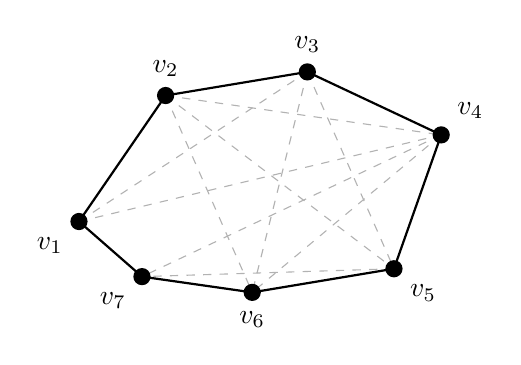
\begin{tikzpicture}[
    city/.style={circle, fill=black, inner sep=2.2pt},
    route/.style={thick},
    alt/.style={gray!60, thin, dashed}
]

\coordinate (A) at (0.2,1.1);
\coordinate (B) at (1.3,2.7);
\coordinate (C) at (3.1,3.0);
\coordinate (D) at (4.8,2.2);
\coordinate (E) at (4.2,0.5);
\coordinate (F) at (2.4,0.2);
\coordinate (G) at (1.0,0.4);

% pomocné spojenia
\draw[alt] (A)--(C);
\draw[alt] (A)--(D);
\draw[alt] (B)--(D);
\draw[alt] (B)--(E);
\draw[alt] (C)--(E);
\draw[alt] (C)--(F);
\draw[alt] (D)--(F);
\draw[alt] (D)--(G);
\draw[alt] (E)--(G);
\draw[alt] (B)--(F);

% výsledná trasa
\draw[route] (A)--(B)--(C)--(D)--(E)--(F)--(G)--(A);

% vrcholy
\node[city,label=below left:$v_1$] at (A) {};
\node[city,label=above:$v_2$] at (B) {};
\node[city,label=above:$v_3$] at (C) {};
\node[city,label=above right:$v_4$] at (D) {};
\node[city,label=below right:$v_5$] at (E) {};
\node[city,label=below:$v_6$] at (F) {};
\node[city,label=below left:$v_7$] at (G) {};

\end{tikzpicture}